\section{Methodology}

\begin{frame}
\begin{center}
     	\huge Methodology
     \end{center}
\end{frame}

\begin{frame}
\frametitle{The Approach}
\begin{figure}
\includegraphics[scale=0.14]{graphics/setup.pdf}
\end{figure}
\note{Feature-based approach}
\end{frame}

\begin{frame}
\frametitle{The Data}
\begin{columns}
	\begin{column}{0.45\textwidth}
		Datasets:
			\begin{itemize}
				\item Facebook - Wall posts from one user to another
				\item Scratch - Comments on uploaded programming projects 
			\end{itemize}
			
		Directed, timestamps.
		\end{column}
		\begin{column}{0.55\textwidth}
			\begin{figure}
				\includegraphics[scale=0.24]{graphics/directed_network.pdf}
			\end{figure}
		\end{column}
	\end{columns}
\end{frame}

\begin{frame}
\frametitle{Snapshot Split-up}
The dataset is split into a total of 26 snapshots:
\begin{itemize}
\item 7 from facebook
\item 19 from Scratch
\end{itemize}

Non-overlapping

Same length = observation window $\Omega$.

Something with node interaction being smaller than Omega. (90th percentile?)


\end{frame}

\begin{frame}
\frametitle{Feature Selection}
12 features based upon the graph.

	\begin{columns}
		\begin{column}{0.5\textwidth}
			\begin{figure}
				\includegraphics[scale=0.27]{graphics/directed_network.pdf}
			\end{figure}
		\end{column}
		\begin{column}{0.5\textwidth}
			\begin{table}
				\begin{tabular}{"l"}
				\thinhline
					In-degree				\\ \thinhline
					Out-degree				\\ \thinhline
					Weighted in-degree		\\ \thinhline
					Weighted out-degree		\\ \thinhline
					Reciprocity				\\ \thinhline
					New activity			\\ \thinhline
					Social strategy			\\ \thinhline
					Betweenness centrality	\\ \thinhline
					PageRank				\\ \thinhline
					Weighted PageRank		\\ \thinhline
					Transitivity			\\ \thinhline
					Weighted transitivity 	\\ \thinhline
				\end{tabular}
			\end{table}
		\end{column}
	\end{columns}

\end{frame}

\begin{frame}
\frametitle{Feature Example}


\begin{columns}
		\begin{column}{0.5\textwidth}
			\begin{figure}
				\includegraphics[scale=0.27]{graphics/directed_network_example.pdf}
			\end{figure}
		\end{column}
		\begin{column}{0.5\textwidth}
			\begin{table}
				\begin{tabular}{"l"l"}
				\thinhline
					In-degree				& 5		\\ \thinhline
					Out-degree				& 4		\\ \thinhline
					Weighted in-degree		& 36	\\ \thinhline
					Weighted out-degree		& 32	\\ \thinhline
					Reciprocity				& 4		\\ \thinhline
					New activity			& 0		\\ \thinhline
					Social strategy			& 0		\\ \thinhline
					Betweenness centrality	& 38.7		\\ \thinhline
					PageRank				& 0.21	\\ \thinhline
					Weighted PageRank		& -		\\ \thinhline
					Transitivity			& $\frac{1}{3}$		\\ \thinhline
					Weighted transitivity 	& -		\\ \thinhline
				\end{tabular}
			\end{table}
		\end{column}
	\end{columns}

\end{frame}

\begin{frame}
\frametitle{Role Discovery and Membership}

\begin{columns}
	\begin{column}{0.5\textwidth}
		\begin{block}{\small Non-negative Matrix Factorization}
			$X \approx UV$
		\end{block}
	\end{column}
	\begin{column}{0.5\textwidth}
	\end{column}
\end{columns}
\begin{figure}
\includegraphics[scale=.3]{graphics/nmf}
\end{figure}

\begin{itemize}
\item Matrix U is role features 
\item Matrix V is membership weights for the roles for each user
\end{itemize}
\note{
\begin{itemize}
\item Frobenius NMF updated with euclidean distance
\item U and V are initialized with left and right matrix from nndsvd (Modified svd)

\end{itemize}
}
\end{frame}

\begin{frame}
\frametitle{Selection of L}
\begin{block}{\small Root Mean Squired Error}
$RMSE = \sqrt{\frac{1}{|X|} \sum\limits_{(u,f) \in X}(X_{u,f}-X'_{u,f})}$
\end{block}

\begin{columns}
	\begin{column}{0.5\textwidth}
	\begin{figure}\caption{Facebook}
		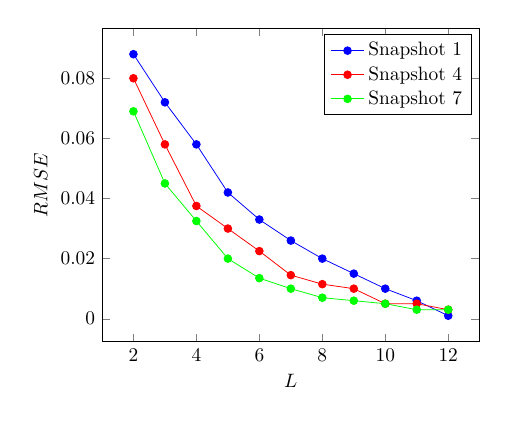
\begin{tikzpicture}[scale=0.7]
    \begin{axis}[
    	scaled ticks=false, 
    	tick label style={/pgf/number format/fixed},
        xlabel=$L$,
        ylabel=$RMSE$]
    \addplot[mark=*,blue] plot coordinates {
        (2, 0.088)
        (3, 0.072)
        (4, 0.058)
        (5, 0.042)
        (6, 0.033)
        (7, 0.026)
        (8, 0.020)
        (9, 0.015)
        (10, 0.010)
        (11, 0.006)
        (12, 0.001)
    };
    \addlegendentry{Snapshot 1}

    \addplot[color=red,mark=*]
        plot coordinates {
        (2, 0.08)
        (3, 0.058)
        (4, 0.0375)
        (5, 0.030)
        (6, 0.0225)
        (7, 0.0145)
        (8, 0.0115)
        (9, 0.01)
        (10, 0.005)
        (11, 0.005)
        (12, 0.003)
        };
    \addlegendentry{Snapshot 4}
    
    \addplot[color=green,mark=*]
        plot coordinates {
        (2, 0.069)
        (3, 0.045)
        (4, 0.0325)
        (5, 0.020)
        (6, 0.0135)
        (7, 0.010)
        (8, 0.007)
        (9, 0.006)
        (10, 0.005)
        (11, 0.003)
        (12, 0.003)
        };
    \addlegendentry{Snapshot 7}
    \end{axis}
\end{tikzpicture}	
\end{figure}
	\end{column}
	
	\begin{column}{0.5\textwidth}
	\begin{figure}\caption{Scratch}
		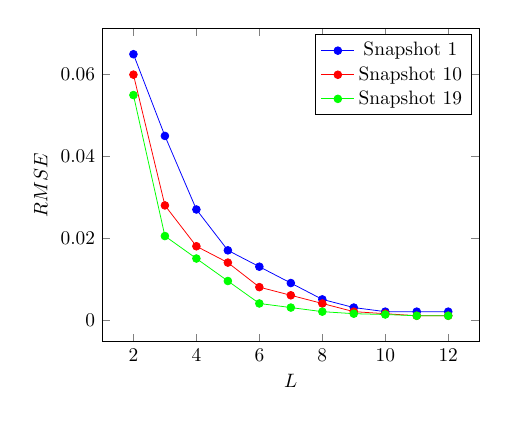
\begin{tikzpicture}[scale=0.7]
    \begin{axis}[
    	scaled ticks=false, 
    	tick label style={/pgf/number format/fixed},
        xlabel=$L$,
        ylabel=$RMSE$]
    \addplot[mark=*,blue] plot coordinates {
        (2, 0.065)
        (3, 0.045)
        (4, 0.027)
        (5, 0.017)
        (6, 0.013)
        (7, 0.009)
        (8, 0.005)
        (9, 0.003)
        (10, 0.002)
        (11, 0.002)
        (12, 0.002)
    };
    \addlegendentry{Snapshot 1}

    \addplot[color=red,mark=*]
        plot coordinates {
        (2, 0.06)
        (3, 0.028)
        (4, 0.018)
        (5, 0.014)
        (6, 0.008)
        (7, 0.006)
        (8, 0.004)
        (9, 0.002)
        (10, 0.0015)
        (11, 0.001)
        (12, 0.001)
    };
    \addlegendentry{Snapshot 10}
    
    \addplot[color=green,mark=*]
        plot coordinates {
        (2, 0.055)
        (3, 0.0205)
        (4, 0.015)
        (5, 0.0095)
        (6, 0.004)
        (7, 0.003)
        (8, 0.002)
        (9, 0.0015)
        (10, 0.0013)
        (11, 0.001)
        (12, 0.001)
        };
    \addlegendentry{Snapshot 19}
    \end{axis}
\end{tikzpicture}	
\end{figure}
	\end{column}
\end{columns}

\end{frame}

\begin{frame}
\frametitle{Tracing Roles}
The sim between snapshots. 
\end{frame}